% Copyright (c) 2018-2020 Craig Ferguson <me@craigfe.io>
% 
% Permission to use, copy, modify, and distribute this software for any
% purpose with or without fee is hereby granted, provided that the above
% copyright notice and this permission notice appear in all copies.
% 
% THE SOFTWARE IS PROVIDED "AS IS", WITHOUT WARRANTY OF ANY KIND, EXPRESS OR
% IMPLIED, INCLUDING BUT NOT LIMITED TO THE WARRANTIES OF MERCHANTABILITY,
% FITNESS FOR A PARTICULAR PURPOSE AND NONINFRINGEMENT. IN NO EVENT SHALL THE
% AUTHORS OR COPYRIGHT HOLDERS BE LIABLE FOR ANY CLAIM, DAMAGES OR OTHER
% LIABILITY, WHETHER IN AN ACTION OF CONTRACT, TORT OR OTHERWISE, ARISING FROM,
% OUT OF OR IN CONNECTION WITH THE SOFTWARE OR THE USE OR OTHER DEALINGS IN THE
% SOFTWARE.

\documentclass[12pt,tikz,margin=5mm]{standalone}

\usetikzlibrary{backgrounds}
\usetikzlibrary{positioning}
\usetikzlibrary{calc}
\usetikzlibrary{decorations.pathreplacing}

% ------------------------------------------------------------------------------
% Typesetting
% ------------------------------------------------------------------------------

\usepackage[T1]{fontenc}
\usepackage{fontspec}

\usepackage{lmodern} % loaded for sans serif
\usepackage[nottdefault,scale=0.9,otf]{sourcecodepro}
\usepackage[scaled=0.96,osf,tighter]{newpxtext}
\linespread{1.05} % Maintain 12pt line spacing

\setsansfont{Latin Modern Sans}
\renewcommand*{\ttdefault}{npxtt}

% The Tableau20 colours
\definecolor{TabLightOrange}{RGB}{255,187,120}
\definecolor{TabOrange}{RGB}{255,127,14}
\definecolor{TabLightBlue}{RGB}{174,199,232}
\definecolor{TabBlue}{RGB}{31,119,180}
\definecolor{TabGreen}{RGB}{44,160,44}
\definecolor{TabLightGreen}{RGB}{152,223,138}
\definecolor{TabSalmon}{RGB}{255,152,150}
\definecolor{TabRed}{RGB}{214,39,40}
\definecolor{TabPurple}{RGB}{148,103,189}
\definecolor{TabLightPurple}{RGB}{197,176,213}
\definecolor{TabLightPink}{RGB}{247,182,210}
\definecolor{TabPink}{RGB}{227,119,194}
\definecolor{TabLightBrown}{RGB}{196,156,148}
\definecolor{TabBrown}{RGB}{140,86,75}
\definecolor{TabGray}{RGB}{127,127,127}
\definecolor{TabOlive}{RGB}{188,189,34}
\definecolor{TabLightOlive}{RGB}{219,219,141}
\definecolor{TabLightGray}{RGB}{199,199,199}
\definecolor{TabLightCyan}{RGB}{158,218,229}
\definecolor{TabCyan}{RGB}{23,190,207}

% ------------------------------------------------------------------------------
% Spacing
% ------------------------------------------------------------------------------

\def\storespace{0.5}
\def\boxspace{0.3}
\def\commitwidth{2cm}
\def\commitheight{1cm}
\def\blobwidth{7mm}
\def\blobheight{7mm}

\tikzstyle{arrow} = [thick,->,>=stealth]

\newcommand{\tikzmark}[2][]{%
  \tikz[remember picture,overlay]\coordinate[#1](#2);%
}

\renewcommand*{\ttdefault}{npxtt}

\def\blockcolor{black!70}
\begin{document}
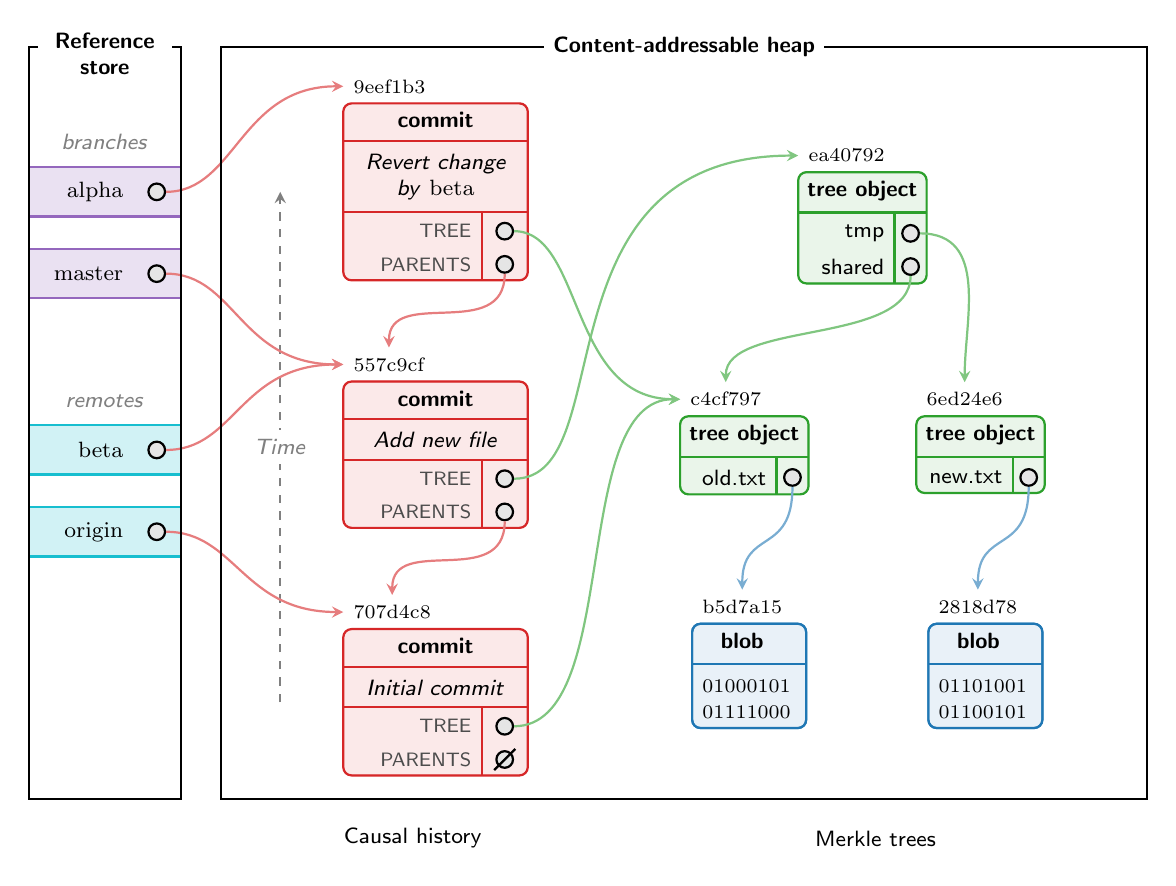
\begin{tikzpicture}
  [ remember picture
  , every node/.style={font=\footnotesize\sffamily}
  , hashcirc/.style={draw=black, fill=black!10, circle, inner sep=0pt, minimum size=6pt}
  , hash/.style={font=\scriptsize\ttfamily}
  , commit/.style = {
    , rectangle
    , rounded corners
    , inner sep = 0
    , fill=TabRed!5
    , draw=\blockcolor
    , line width=0.75pt,
    , minimum width=\commitwidth
    , minimum height = \commitheight
  }
  , gitptr/.style={draw=TabBlue!60}
  , arrow={->,>=stealth}
  ]

  \def\linespacing{15pt}
  \def\commit[#1]#2(#3)#4(#5)#6(#7) {
    \begin{scope}[local bounding box=#1]
      \begin{scope}[local bounding box=inner-#1]
        \node (#1-init) at (#3) {\textbf{commit}};
        \node[text width = 6em, align=center, below=\linespacing of #1-init.north, anchor=north] (#1-2) {\emph{#5}};
      \end{scope}

      \coordinate (mid) at ($ (#1-init.south)!0.5!(#1-2.north) $);
      \coordinate (triple) at ($ (inner-#1.west |- 0, 0 |- mid)!0.75!(inner-#1.east |- 0, 0 |- mid) $);
      
      \coordinate[below=0.5*\linespacing of #1-2.south] (x);
      \node[anchor=east, text=black!70] at (triple |- 0, 0 |- x) (#1-tree-label) {\scriptsize TREE};
      \coordinate (x) at ($ (#1-tree-label) + (0, -0.8*\linespacing) $);
      \node[anchor=east, text=black!70] at (triple |- 0, 0 |- x) (#1-parent-label) {\scriptsize PARENTS};
    \end{scope}
    
    \draw[-, TabRed] (#1.west |- 0, 0 |- mid) -- (#1.east |- 0, 0 |- mid);
    \coordinate (mid) at ($ (#1-2.south)!0.5!(#1-tree-label.north) $);
    \draw[-, TabRed] (#1.west |- 0, 0 |- mid) -- (#1.east |- 0, 0 |- mid);
    \coordinate (triple) at ($ (inner-#1.south west |- 0, 0 |- mid)!0.75!(inner-#1.south east |- 0, 0 |- mid) $);
    
    \draw[-, TabRed] (triple) -- (triple |- 0, 0 |- #1.south);
    \draw [draw=TabRed, rounded corners=.3em] (#1.north west) rectangle (#1.south east);

    \begin{scope}[on background layer]
      \draw [fill=TabRed!10, draw=TabRed, rounded corners=.3em] (#1.north west) rectangle (#1.south east);
    \end{scope}
    
    \node[anchor=south west, hash] (#1-hash) at ($ (#1.north west) $) {#7};

    \coordinate (x) at ($ (triple)!0.5!(#1.east) $);
    \node[hashcirc] (#1-tree) at (x |- 0,
0 |- #1-tree-label) {};
    
    \node[hashcirc] (#1-parent) at (x |-
0, 0 |- #1-parent-label) {};
  }
  
  \def\treecolor{TabGreen}
  \def\tree[#1]#2(#3)#4(#5)#6(#7) {
    \begin{scope}[local bounding box=#1]
      \begin{scope}[local bounding box=inner-#1]
        \node (#1-init) at (#3) {\raisebox{2pt}{\textbf{tree object}}};
      \end{scope}

      \coordinate (mid) at ($ (#1-init) $);
      \coordinate (triple) at ($ (inner-#1.west |- 0, 0 |- mid)!0.75!(inner-#1.east |- 0, 0 |- mid) $);
      
      \coordinate (x) at ($ (#1-init) + (0, -\linespacing) $);
      \node[anchor=east] at (triple |- 0, 0 |- x) (#1-tree-label) {\footnotesize \textsf{tmp}};
      \coordinate (x) at ($ (#1-tree-label) + (0, -0.8*\linespacing) $);
      \node[anchor=east] at (triple |- 0, 0 |- x) (#1-parent-label) {\footnotesize \textsf{shared}};
    \end{scope}
    
    \coordinate (mid) at ($ (#1-init)!0.5!(#1-tree-label) $);
    \draw[-, \treecolor] (#1.west |- 0, 0 |- mid) -- (#1.east |- 0, 0 |- mid);
    \coordinate (triple) at ($ (inner-#1.west |- 0, 0 |- mid)!0.75!(inner-#1.east |- 0, 0 |- mid) $);
    
    \draw[-, \treecolor] (triple) -- (triple |- 0, 0 |- #1.south);
    \draw [draw=\treecolor, rounded corners=.3em] (#1.north west) rectangle (#1.south east);

    \begin{scope}[on background layer]
      \draw [fill=\treecolor!10, draw=\treecolor, rounded corners=.3em] (#1.north west) rectangle (#1.south east);
    \end{scope}
    
    \node[anchor=south west, hash] (#1-hash) at ($ (#1.north west) $) {#5};

    \coordinate (x) at ($ (triple)!0.5!(#1.east) $);
    \node[hashcirc] (#1-tree) at (x |- 0,
0 |- #1-tree-label) {};
    
    \node[hashcirc] (#1-parent) at (x |-
0, 0 |- #1-parent-label) {};
}

  \def\treesmall[#1]#2(#3)#4(#5)#6(#7) {
    \begin{scope}[local bounding box=#1]
      \begin{scope}[local bounding box=inner-#1]
        \node (#1-init) at (#3) {\raisebox{2pt}{\textbf{tree object}}};
      \end{scope}

      \coordinate (mid) at ($ (#1-init) $);
      \coordinate (triple) at ($ (inner-#1.west |- 0, 0 |- mid)!0.75!(inner-#1.east |- 0, 0 |- mid) $);
      
      \coordinate (x) at ($ (#1-init) + (0, -\linespacing) $);
      \node[anchor=east] at (triple |- 0, 0 |- x) (#1-tree-label) {\footnotesize \textsf{#7}};
    \end{scope}
    
    \coordinate (mid) at ($ (#1-init)!0.5!(#1-tree-label) $);
    \draw[-, \treecolor] (#1.west |- 0, 0 |- mid) -- (#1.east |- 0, 0 |- mid);
    \coordinate (triple) at ($ (inner-#1.west |- 0, 0 |- mid)!0.75!(inner-#1.east |- 0, 0 |- mid) $);
    
    \draw[-, \treecolor] (triple) -- (triple |- 0, 0 |- #1.south);
    \draw [draw=\treecolor, rounded corners=.3em] (#1.north west) rectangle (#1.south east);

    \begin{scope}[on background layer]
      \draw [fill=\treecolor!10, draw=\treecolor, rounded corners=.3em] (#1.north west) rectangle (#1.south east);
    \end{scope}
    
    \node[anchor=south west, hash] (#1-hash) at ($ (#1.north west) $) {#5};

    \coordinate (x) at ($ (triple)!0.5!(#1.east) $);
    \node[hashcirc] (#1-tree) at (x |- 0,
0 |- #1-tree-label) {};
}

  \def\blobcolor{TabBlue}
  \def\blob[#1]#2(#3)#4(#5)#6(#7) {
    \begin{scope}[local bounding box=#1]
      \begin{scope}[local bounding box=inner-#1]
        \node (#1-init) at (#3) {\ \ \,\textbf{blob}};
      \end{scope}

      \coordinate (triple) at ($ (inner-#1.west |- 0, 0 |- #1-init) $);
      \coordinate (x) at ($ (#1-init) + (0, -0.7*\linespacing) $);
      \node[anchor=north west, text width = 1.2cm] at (triple |- 0, 0 |- x) (#1-tree-label) {\scriptsize\texttt{#7}};
      \coordinate (x) at ($ (#1-tree-label) + (0, -0.8*\linespacing) $);
    \end{scope}
    
    \coordinate (mid) at ($ (#1-init.south)!0.5!(#1-tree-label.north) $);
    \draw[-, \blobcolor] (#1.west |- 0, 0 |- mid) -- (#1.east |- 0, 0 |- mid);
    \coordinate (triple) at ($ (inner-#1.west |- 0, 0 |- mid)!0.75!(inner-#1.east |- 0, 0 |- mid) $);
    \draw [draw=\blobcolor, rounded corners=.3em] (#1.north west) rectangle (#1.south east);

    \begin{scope}[on background layer]
      \draw [fill=\blobcolor!10, draw=\blobcolor, line width=0.75pt, rounded corners=.3em] (#1.north west) rectangle (#1.south east);
    \end{scope}
    
    \node[anchor=south west, hash] (#1-hash) at ($ (#1.north west) $) {#5};
  }
  
  \begin{scope}[local bounding box = heap]
    \begin{scope}[local bounding box = commits]

      \commit[c1] (0, 0) (Revert change \\ by \normalfont{\texttt{beta}}) (9eef1b3)

      \coordinate[below = 1.5cm of c1] (commit-2);
      \commit[c2] (commit-2) (Add new file) (557c9cf)

      \coordinate[below = 1.5cm of c2] (commit-3);
      \commit[c3] (commit-3) (Initial commit) (707d4c8)

      \draw[gray, dashed, ->] ($ (c3.west) + (-0.8, 0) $) -- node[midway, fill=white] {\emph{Time}} ($ (c1.west) + (-0.8, 0) $);
    \end{scope}
      
      \coordinate[right=4.25cm of c1] (tree-1);
      \tree[t1] (tree-1) (ea40792) (        
)

      \coordinate[below left=3.1cm and 1.5cm of tree-1] (tree-2);
      \treesmall[t2] (tree-2) (c4cf797) (old.txt)
      
      \coordinate[below right=3.1cm and 1.5cm of tree-1] (tree-3);
      \treesmall[t3] (tree-3) (6ed24e6) (new.txt)
      
      \coordinate[below=2.6cm of tree-2, xshift=-1.5mm] (blob-1);
      \blob[b1] (blob-1) (b5d7a15) (01000101 01111000)

      \coordinate[below=2.6cm of tree-3, xshift=-1.5mm] (blob-2);
      \blob[b2] (blob-2) (2818d78) (01101001 01100101)
      
      \draw[->, gitptr, draw=TabRed!60] (c1-parent) .. controls ++(0, -1) and ++(0, 1) .. (c2-hash);
      \draw[->, gitptr, draw=TabRed!60] (c2-parent) .. controls ++(0, -1) and ++(0, 1) .. (c3-hash);
      \draw[->, gitptr, draw=TabGreen!60] (c1-tree) .. controls ++(1, 0) and ++(-2, 0) .. (t2-hash);
      \draw[->, gitptr, draw=TabGreen!60] (c2-tree) .. controls ++(1.5, 0) and ++(-4, 0) .. (t1-hash);
      \draw[->, gitptr, draw=TabGreen!60] (c3-tree) .. controls ++(1.5, 0) and ++(-2, 0) .. (t2-hash);
      
      \draw[->, gitptr, draw=TabGreen!60] (t1-tree) .. controls ++(1, 0) and ++(0, 1) .. (t3-hash);
      \draw[->, gitptr, draw=TabGreen!60] (t1-parent) .. controls ++(0, -1) and ++(0, 1) .. (t2-hash);
      
      \draw[->, gitptr, draw=TabBlue!60] (t2-tree) .. controls ++(0, -1) and ++(0, 1) .. (b1-hash);
      \draw[->, gitptr, draw=TabBlue!60] (t3-tree) .. controls ++(0, -1) and ++(0, 1) .. (b2-hash);

      \draw [-] ($ (c3-parent.south west) + (-0.05, -0.05) $) -- ($ (c3-parent.north east) + (0.05, 0.05) $);
\end{scope}

\begin{scope}[local bounding box=refs]
  
  \coordinate (t) at (commits.west |- 0, 0 |- c1);
  
  \node[hashcirc, left = 10mm of t] (r-master-hash) {};
  \node[left = 5pt of r-master-hash, minimum height=1.7em, font=\footnotesize\ttfamily] (r-master) {alpha};

  \node[hashcirc, below = 0.8cm of r-master-hash] (r-client-hash) {};
  \node[left = 5pt of r-client-hash, minimum height=1.7em, font=\footnotesize\ttfamily] (r-client) {master};

  \node[hashcirc, below = 2cm of r-client-hash] (r-foo-hash) {};
  \node[left = 5pt of r-foo-hash, minimum height=1.7em, font=\footnotesize\ttfamily] (r-foo) {beta};
  
  \node[hashcirc, below = 0.8cm of r-foo-hash] (r-bar-hash) {};
  \node[left = 5pt of r-bar-hash, minimum height=1.7em, font=\footnotesize\ttfamily] (r-bar) {origin};
\end{scope}

\coordinate (ref-mid) at ($ (refs.west)!0.5!(refs.east) $);
\node[anchor=south,yshift=0.1cm,gray] (branch-label) at (ref-mid |- 0, 0 |- r-master.north) {\emph{branches}};

\node[anchor=south,yshift=0.1cm,gray] (remote-label) at (ref-mid |- 0, 0 |- r-foo.north) {\emph{remotes}};

\draw[->, gitptr, draw=TabRed!60] (r-master-hash) .. controls ++(1, 0) and ++(-1.9, 0) .. (c1-hash);
\draw[->, gitptr, draw=TabRed!60] (r-client-hash) .. controls ++(1, 0) and ++(-1.9, 0) .. (c2-hash);
\draw[->, gitptr, draw=TabRed!60] (r-foo-hash) .. controls ++(1, 0) and ++(-1.9, 0) .. (c2-hash);
\draw[->, gitptr, draw=TabRed!60] (r-bar-hash) .. controls ++(1, 0) and ++(-1.9, 0) .. (c3-hash);

% Compute outer bounding boxes
\coordinate (heap-nw) at ($ (heap.north west) + (-\boxspace, \boxspace) $);
\coordinate (heap-ne) at ($ (heap.north east) + (\boxspace + 1, \boxspace) $);
\coordinate (heap-sw) at ($ (heap.south west) + (-\boxspace, -\boxspace) $);
\coordinate (heap-se) at ($ (heap.south east) + (\boxspace + 1, -\boxspace) $);

\coordinate (divline) at ($(c1.east)!0.5!(t2.west)$);
% \draw[-, dotted, TabGray] (divline |- 0, 0 |- heap-ne) -- (divline |- 0, 0 |- heap-se);
\coordinate (labelheight) at ($(heap-se) + (0, -0.5)$);
\coordinate (causal-label-x) at ($(heap-sw)!0.5!(divline)$);
\coordinate (merkle-label-x) at ($(heap-se)!0.5!(divline)$);
\node[rectangle, fill=white] at (causal-label-x |- 0, |- labelheight) {Causal history};
\node[rectangle, fill=white] at (merkle-label-x |- 0, |- labelheight) {Merkle trees};

\def\refsinnerpad{0.2}

\coordinate (east-bound) at ($ (refs.east) + (\refsinnerpad, 0) $);
\coordinate (west-bound) at ($ (refs.west) + (-\refsinnerpad, 0) $);

\coordinate (refs-nw) at (west-bound |- 0, 0 |- heap-nw);
\coordinate (refs-ne) at  (east-bound |- 0, 0 |- heap-nw);
\coordinate (refs-sw) at (west-bound |- 0, 0 |- heap-sw);
\coordinate (refs-se) at (east-bound |- 0, 0 |- heap-sw);

\foreach \x in {r-master,r-client} {
  \draw[-, TabPurple] (refs-sw |- 0, 0 |- \x.north) -- (refs-se |- 0, 0 |- \x.north);
  \draw[-, TabPurple] (refs-sw |- 0, 0 |- \x.south) -- (refs-se |- 0, 0 |- \x.south);
  \begin{scope}[on background layer]
    \draw[draw=none, fill=TabPurple!20] (refs-sw |- 0, 0 |- \x.north) rectangle (refs-se |- 0, 0 |- \x.south);
  \end{scope}
}

\foreach \x in {r-foo,r-bar} {
  \draw[-, TabCyan] (refs-sw |- 0, 0 |- \x.north) -- (refs-se |- 0, 0 |- \x.north);
  \draw[-, TabCyan] (refs-sw |- 0, 0 |- \x.south) -- (refs-se |- 0, 0 |- \x.south);
  \begin{scope}[on background layer]
    \draw[draw=none, fill=TabCyan!20] (refs-sw |- 0, 0 |- \x.north) rectangle (refs-se |- 0, 0 |- \x.south);
  \end{scope}
}

\draw[draw, thick] (heap-nw) rectangle (heap-se);
\draw[draw, thick] (refs-nw) rectangle (refs-se);

\node[rectangle, fill=white] at ($(heap-nw)!0.5!(heap-ne)$) (heap-label) {\textbf{Content-addressable heap}};

\node[anchor=north, yshift=5pt, fill=white, text width=1.7cm, outer sep=0, inner sep=0, align=center] at
($(refs-nw)!0.5!(refs-ne)$) (refs-label) {\textbf{Reference\\ store}};

\end{tikzpicture}
\end{document}
